\documentclass[12pt,a4paper,twoside]{article}
\usepackage{labor}
\begin{document}

%fill for cover and header creation
\newcommand\laboratorynumber{2}
\title{Mikroskop}
\newcommand\supervisor{Nico Knefz}
\newcommand\groupnumber{42}

\newcommand\participantonelastname{Eisner}
\newcommand\participantonefirstname{Nico}
\newcommand\participantoneid{12214121}
\newcommand\participanttwolastname{Waldl}
\newcommand\participanttwofirstname{Philip}
\newcommand\participanttwoid{12214120}
\author{\participantonelastname \ \& \participanttwolastname}

\newcommand\degreeid{UB 033 678}
\newcommand\semester{23WS}
\date{13.10.2023}

%select correct course title
%\newcommand\coursetitle{Einführung in die \\ physikalischen Messmethoden}
%\newcommand\coursetitle{Laborübungen 1: \\ Mechanik und Wärme}
\newcommand\coursetitle{Laborübungen 2: \\ Elektrizität, Magnetismus, Optik}
%\newcommand\coursetitle{Fortgeschrittenen Praktikum 1: \\ Technische Physik}
%\newcommand\coursetitle{Fortgeschrittenen Praktikum 2: \\ Allgemeine Physik}

%\begin{titlepage}
   \begin{center}
       \begin{figure}[H]
            \begin{minipage}[h]{30mm}
                \centerline{
\includegraphics[height=15mm]{cover_nudes/tugraz.png}}
            \end{minipage}
            \hfill
            \begin{minipage}[h]{30mm}
                \centerline{
\includegraphics[height=15mm]{cover_nudes/nawi_graz.png}}
            \end{minipage}
            \hfill
            \begin{minipage}[h]{30mm}
                \centerline{
\includegraphics[height=15mm]{cover_nudes/uni-graz.png}}
            \end{minipage}
        \end{figure}
        
        \large{\emph{Institut für Experimentalphysik der Technischen Universität Graz \\
        \& Institut für Physik der Universität Graz}} \\
        \vspace{5mm}
        
        {\Huge \textbf{\coursetitle}}
        \vspace{5mm}
        
        {\huge \laboratorynumber: \thetitle}
    \end{center}
    
    \vfill
    
    \begin{table}[H]
        \LARGE
        \centering
        \begin{tabular}{r l}
            Betreuer:       & \supervisor \\
            Gruppennummer:  & \groupnumber \\
            \\
            Name:           & \participantonelastname, \participantonefirstname \\
            Matrikelnummer: & \participantoneid \\
            Name:           & \participanttwolastname, \participanttwofirstname \\
            Matrikelnummer: & \participanttwoid \\
            \\
            Kennzahl:       & \degreeid \\
            Datum:          & \semester \ | \thedate
        \end{tabular}
    \end{table}
    \vspace{4cm}
\end{titlepage}
\clearpage
\setcounter{page}{1}

%\maketitle %short title alternative

\includepdf[pages={1}]{../Deckblätter/DeckBlatt_Mikroskop.pdf}

\tableofcontents
\newpage

\section{Aufgabenstellung} %jo beschreibn wos gmocht host ------------------------------
Das Experiment Mikroskop behandelt die grundlegende Untersuchung mittels Mikroskop. 
Dabei wird vor allem Fokus auf die Vergrößerung gesetzt und ein diesbezüglicher Vergleich zwischen einem altem- und einem neuen Mikroskop beschrieben.
Die genaue Aufgabenstellung des Laborversuches sieht wie folgt aus:

\begin{itemize}
    \item Gesamt- und Objektivvergrößerung des alten Mikroskops für fünf verschiedene Tubuslängen 
    + Diagramm der Gesamtvergrößerung in Abhängigkeit von der mechanischen Tubuslänge 
    $\alpha$
    \item Okularvergrößerung $V_{Ok}$ 
    \item Objektivbrennweite $f_{Obj}$ aus Diagramm
    \item Gesamtvergrößerung des neuen Mikroskops fur alle drei Objektive
    \item Vergleich der beiden Mikroskope
    \item Probenuntersuchung mittels digitalem Mikroskop
\end{itemize}

\noindent
Alle Informationen und Methodiken wurden uns von der Technischen Universität bereitgestellt \cite{teachcenter1}. 


\section{Voraussetzungen \& Grundlagen} %Grundlagen erklären, Formeln mit erklärung

Mikroskope werden in der Regel dazu verwendet, für den Menschen nicht sichtbare Objekte und Stoffe zu Vergrößern und diese schärfstmöglich und gut erkennbar darzustellen.
Im Grunde setzt sich dieses Vergößerungsmittel aus (von unten nach oben) 

\begin{itemize}
    \item Leuchtquelle
    \item Objektträger
    \item Objektiv
    \item Tubus
    \item Okular
\end{itemize}

\noindent
zusammen.

\begin{figure}[H]
    \centering
    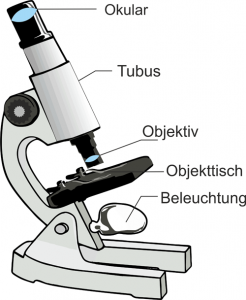
\includegraphics[width=0.3\linewidth]{nudes/mikroskop_aufbau.png}
    \caption{Grundlegender Aufbau eines Mikroskops \cite{mikr_aufbau}}
    \label{fig:Aufbau Mikroskop}
\end{figure}

\noindent
Der grobe Strahlengang sieht dabei wie folgt aus:

\begin{figure}[H]
    \centering
    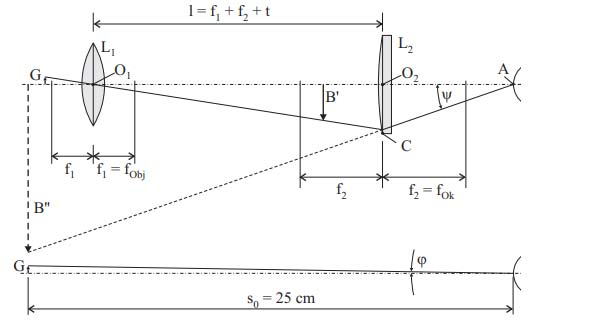
\includegraphics[width=0.7\linewidth]{nudes/StrahlengangMikro.png}
    \caption{Strahlengang Mikroskop \cite{teachcenter1}}
    \label{fig:Strahlengang Mikroskop}
\end{figure}

\noindent
Wie in Abbildung \ref{fig:Strahlengang Mikroskop} ersichtlich, sind die beiden wichtigsten Elemente zur Vergößerung zwei Sammellinsen, das Objektiv und das Okular, dessen Abstand zueinander größer ist, als die Summe ihrer beiden Brennweiten $f_{1}$ und $f_{2}$. 
Dadurch entsteht ein reelles, umgekehrtes Bild B' innerhalb der Brennweite $f_{2}$ des Okulars, und weiters ein sehr stark vergößertes, virutelles Bild B'' innerhalb der Sehweite des Auges $s_{0}$. Der Gegenstand befindet sich dabei dicht an der Objektivbrennweite $f_{1}$. \newline

\noindent
Um nun die als Verhältnis des Sehwinkels mit Instrument, zum Sehwinkel ohne Instrument definierte gesamte Vergrößerung zu erhalten, kann die Formel

    \begin{equation}
        \label{eq:Gesamtvergrößerung}
        \centerline{$V_{ges}=V_{Obj}*V_{Oku}$}
    \end{equation}

    \begin{equation}
        \label{eq:Unsicherheit_Gesamtvergrößerung}
        \centerline{$\Delta V_{ges} = \vert \frac{\partial V_{ges}}{V_{Obj}} * \Delta V_{Obj} \vert + \vert \frac{\partial V_{ges}}{\partial V_{Oku}} * \Delta V_{Oku} \vert$}
    \end{equation}

\noindent
verwendet werde, wobei sich $V_{Obj}$ aus

\begin{equation}
    \label{eq:Objektivvergrößerung}
    \centerline{$V_{Obj}=\frac{t}{f_{1}}$}
\end{equation}

\noindent
und $V_{Oku}$ aus

\begin{equation}
    \label{eq:Okularvergrößerung}
    \centerline{$V_{Oku}=\frac{s_{0}}{f_{2}}$}
\end{equation}

\noindent
zusammen setzt. \newline

\noindent
Die Brennweite $f_{obj}$ des Objektives lösst sich mittels Tubuslänge t und folgender Behauptung bestimmen:

\begin{equation}
    \label{eq:Objektivbrennweite}
    \centerline{$V_{obj}=\frac{V_{ges}}{V_{Oku}}=\frac{t}{f_{Obj}}$}
\end{equation}

\begin{equation}
    \label{eq:Unsicherheit_Objektivbrennweite}
    \centerline{$\Delta V_{obj} = \vert \frac{\partial V_{obj}}{\partial t} * \Delta t \vert + \vert \frac{\partial V_{obj}}{\partial f_{Obj}} * \Delta f_{Obj} \vert $}
\end{equation}

\noindent
Zur Berechnung der jeweiligen Gesamtvergrößerungen werden folgende Formeln verwendet:

\begin{equation}
    \label{eq:VergrößerungAM}
    \centerline{$V=\frac{Vergleichsskala Hinter Mikroskop}{Messkala Am Objekt}$}
\end{equation}

\begin{equation}
    \label{eq:Unsicherheit_VergrößerungAM}
    \centerline{$\Delta V = \vert \frac{\partial V}{\partial VHM} * \Delta VHM \vert + \vert \frac{\partial V}{\partial MAO} * \Delta MAO \vert $}
\end{equation}

\begin{equation}
    \label{eq:VergrößerungAM10x}
    \centerline{$V=\frac{Messkala Am Objekt}{Vergleichsskala Im Okular}$}
\end{equation}

\begin{equation}
    \label{eq:Unsicherheit_VergrößerungAM10x}
    \centerline{$\Delta V = \vert \frac{\partial V}{\partial MAO} * \Delta MAO \vert + \vert \frac{\partial V}{\partial VIO} * \Delta VIO \vert $}
\end{equation}

\begin{equation}
    \label{eq:VergrößerungNM}  
    \centerline{$V=\frac{Vergleichsskala Ober Mikroskop}{Messkala Am Objekt}$}
\end{equation}

\begin{equation}
    \label{eq:Unsicherheit_VergrößerungNM}
    \centerline{$\Delta V = \vert \frac{\partial V}{\partial VOM} * \Delta VOM \vert + \vert \frac{\partial V}{\partial MAO} * \Delta MAO \vert $}
\end{equation}



\section{Versuchsanordnung} %mit skizze kurz beschreiben ------------------------------

    Die wichtigsten Elemente des Versuches lassen sich, abgesehen vom verwendeten Computer, auf das alte- und neue Mikroskop beschränken. \newline
    
    Das ältere Untersuchungswerkzeug lässt sich in folgender Abbildung \ref{fig:Altes Mikroskop} erkennen.  

    \begin{figure}[H]
        \centering
        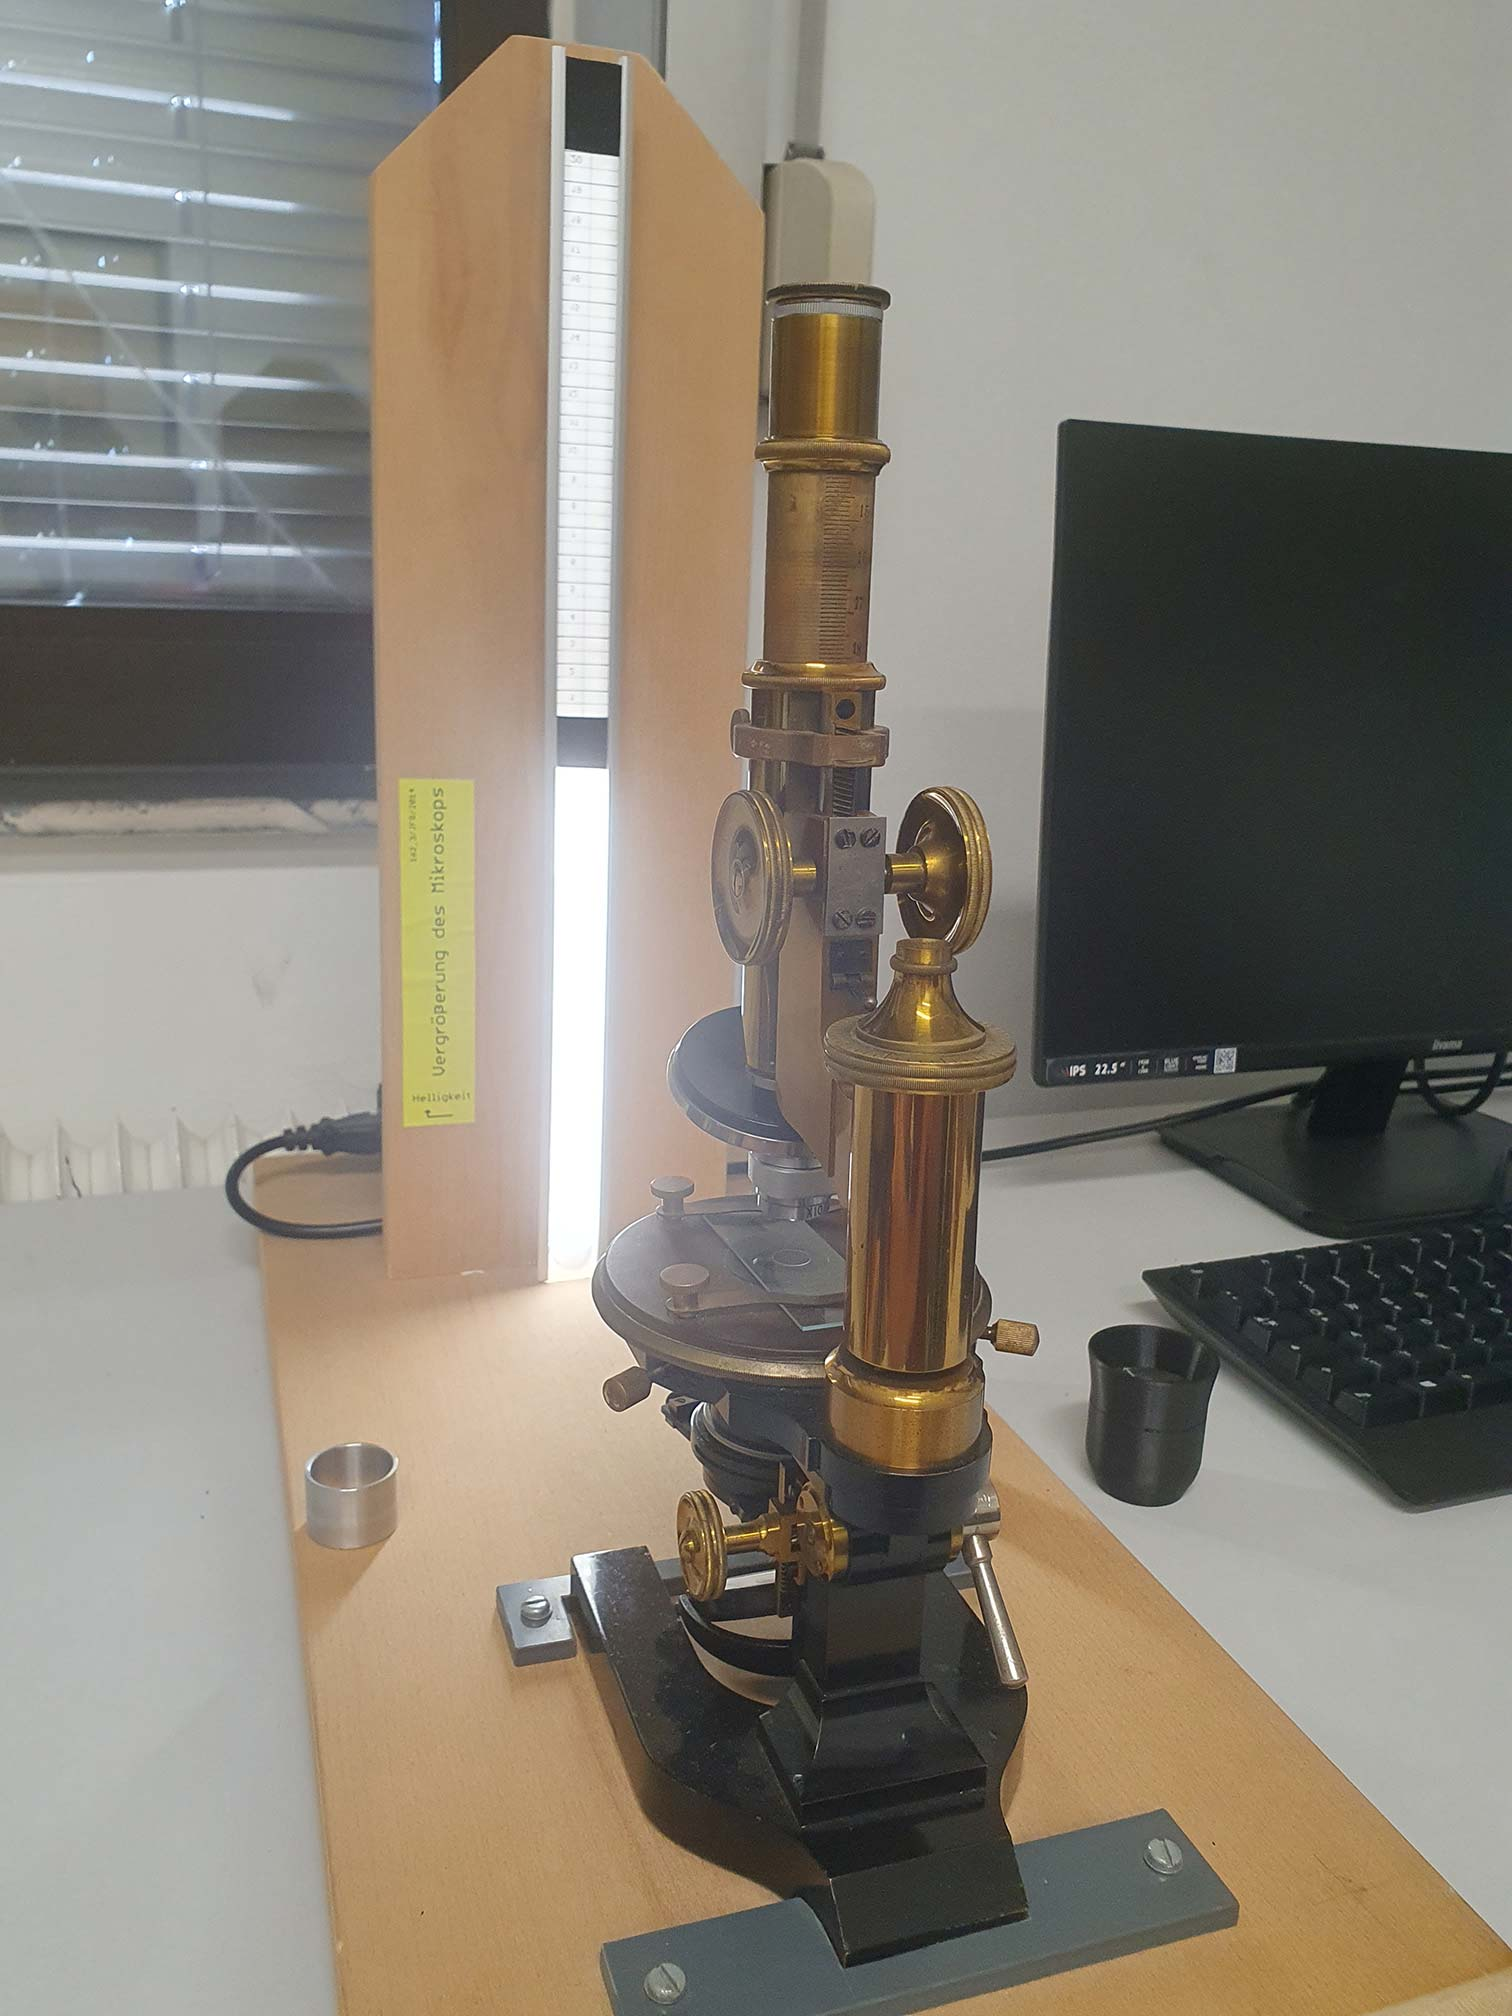
\includegraphics[width=0.5\linewidth, angle=-90]{nudes/AltesMikro.jpg}
        \caption{Altes Mikroskop}
        \label{fig:Altes Mikroskop}
    \end{figure}

    \noindent
    Die Tubuslänge kann hier direkt am Mikroskop mit einem Drehrad verändert werden.
    
    \begin{figure}[H]
        \centering
        \includegraphics[width=0.5\linewidth, angle=-90]{nudes/AltesMikroTubuslänge.jpg}
        \caption{Altes Mikroskop Tubuslänge}
        \label{fig:Altes Mikroskop Tubuslänge}
    \end{figure}

    \noindent
    Um die Vergrößerung bestimmen zu können, muss die Messskala im Okular mit einer realen Skala verglichen werden, wobei sich Letztere beim alten Mikroskop hinter dem Gerät befindet.

    \begin{figure}[H]
        \centering
        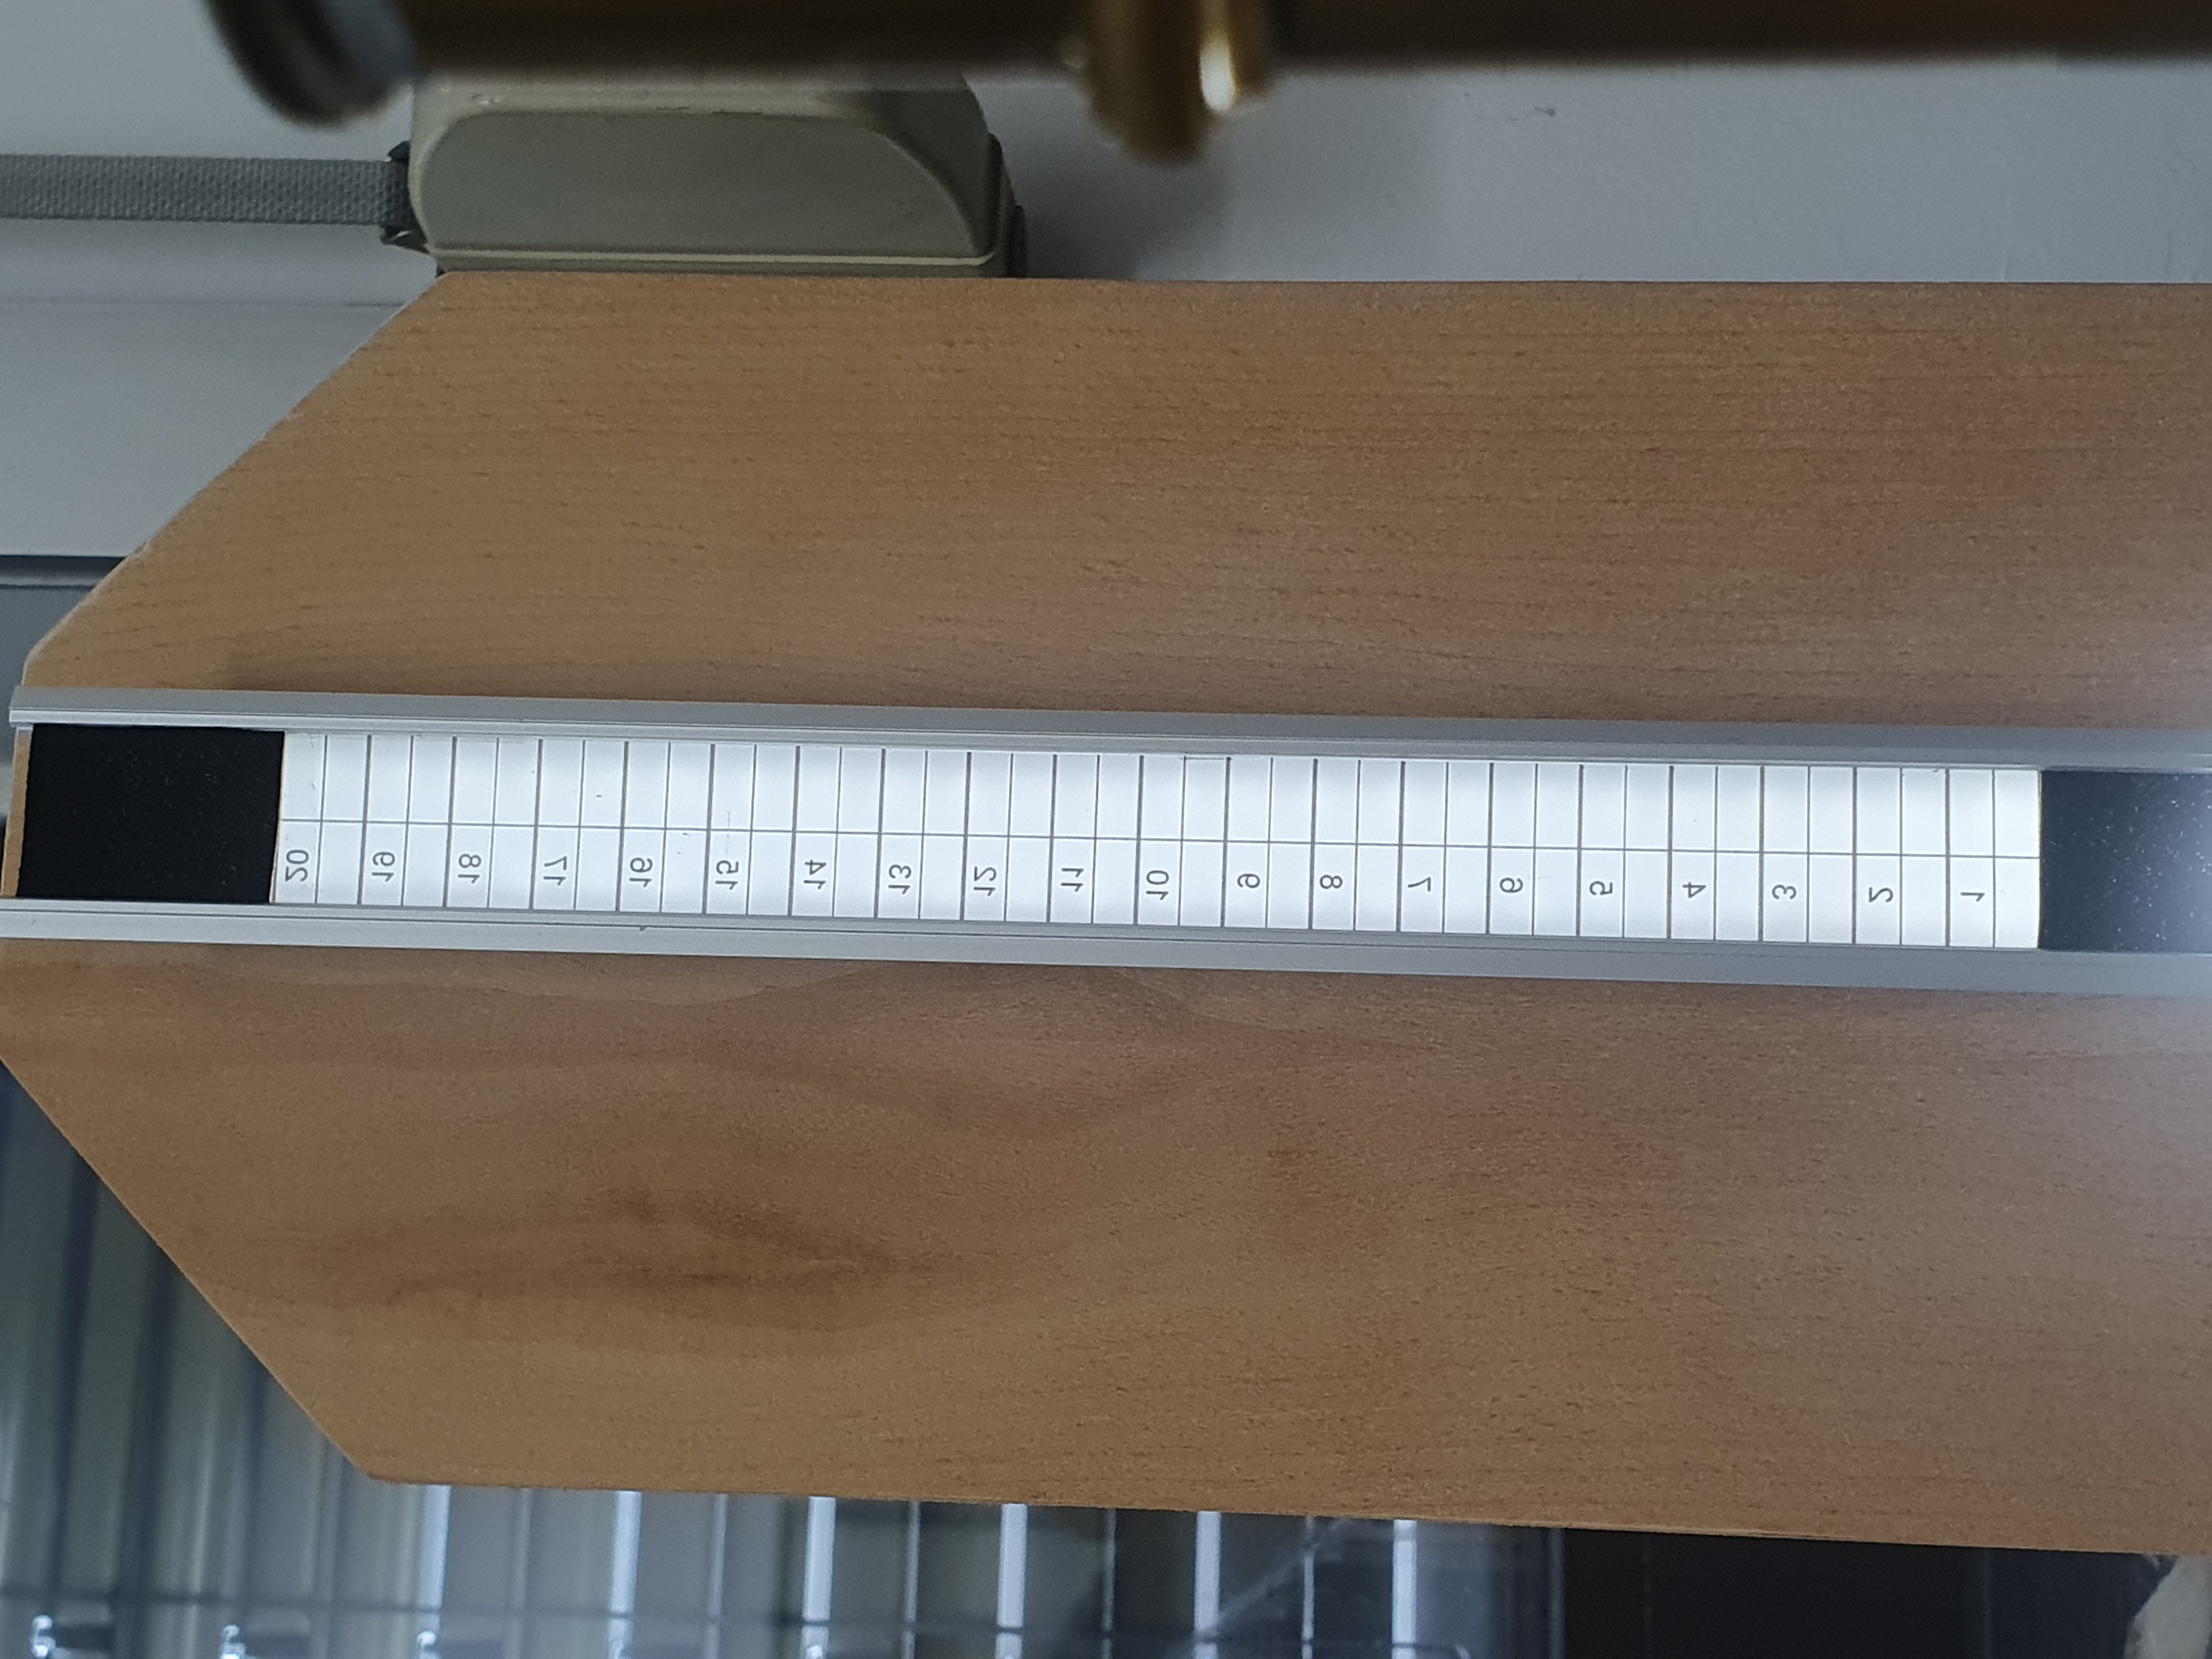
\includegraphics[width=0.5\linewidth, angle=-90]{nudes/AltesMikroMessskala.jpg}
        \caption{Altes Mikroskop Vergleichsskala}
        \label{fig:Altes Mikroskop Skala}
    \end{figure}

    \noindent
    Das neuere Mikroskop sieht dabei etwas kompakter aus und wird in folgender Abbildung \ref{fig:Neues Mirkoskop} abgebildet.

    \begin{figure}[H]
        \centering
        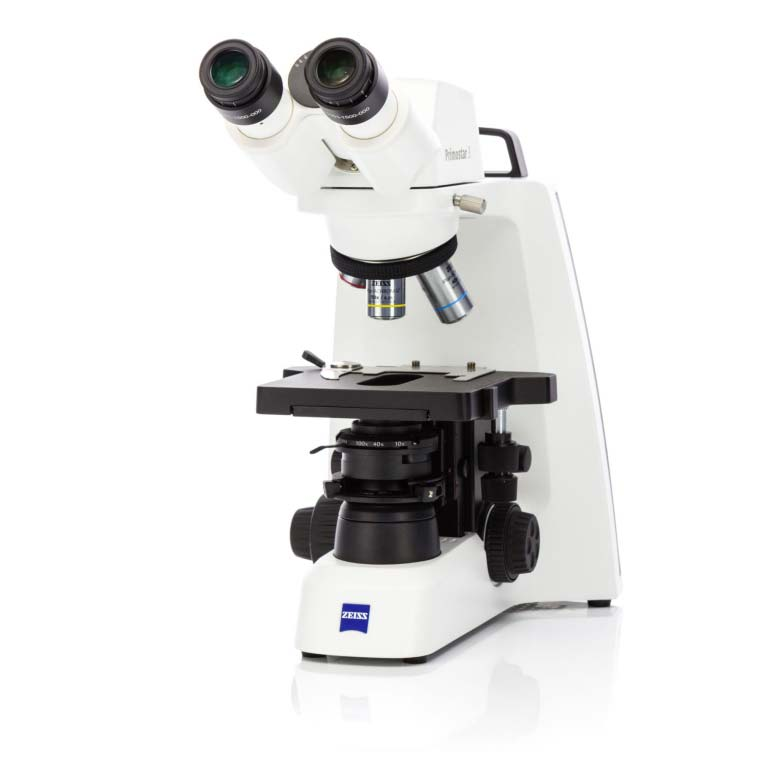
\includegraphics[width=0.5\linewidth, angle=0]{nudes/neues_mikroskop.jpg}
        \caption{Neues Mirkoskop \ref{neues_mikr}}
        \label{fig:Neues Mirkoskop}
    \end{figure}

    \noindent
    Das neuere Hilfsmittel besitzt drei verschiedene Objkektive, zwischen welchen man durch drehen wechseln kann. Weiters wurde an der Oberseite des Mikroskopes eine weitere Vergleichsskala angebracht.
    Mittels Drehräder lassen sich Fokus und Objektposition sehr präzise anpassen. \newline
    
    \noindent
    Außerdem waren aber auch einige kleinere Hilfsmittel vor allem zur Bestimmung der Vergößerungen von Großem Wert. 
    Um die Messskala mit der Objektskala vergleichen zu können, wurde ein Aufsatz mit einem halbdurchlässigem Spiegel verwendet. 
    Durch diesen konnte sowohl die Objektskala, als auch die Messskala hinter (altes Mikroskop) bzw. oberhalb (neues Mikroskop) überlagernd beobachtet werden, was mit Blick auf Abbildung \ref*{fig:Aufsatz} bildlich veranschaulicht wird.

    \begin{figure}[H]
        \centering
        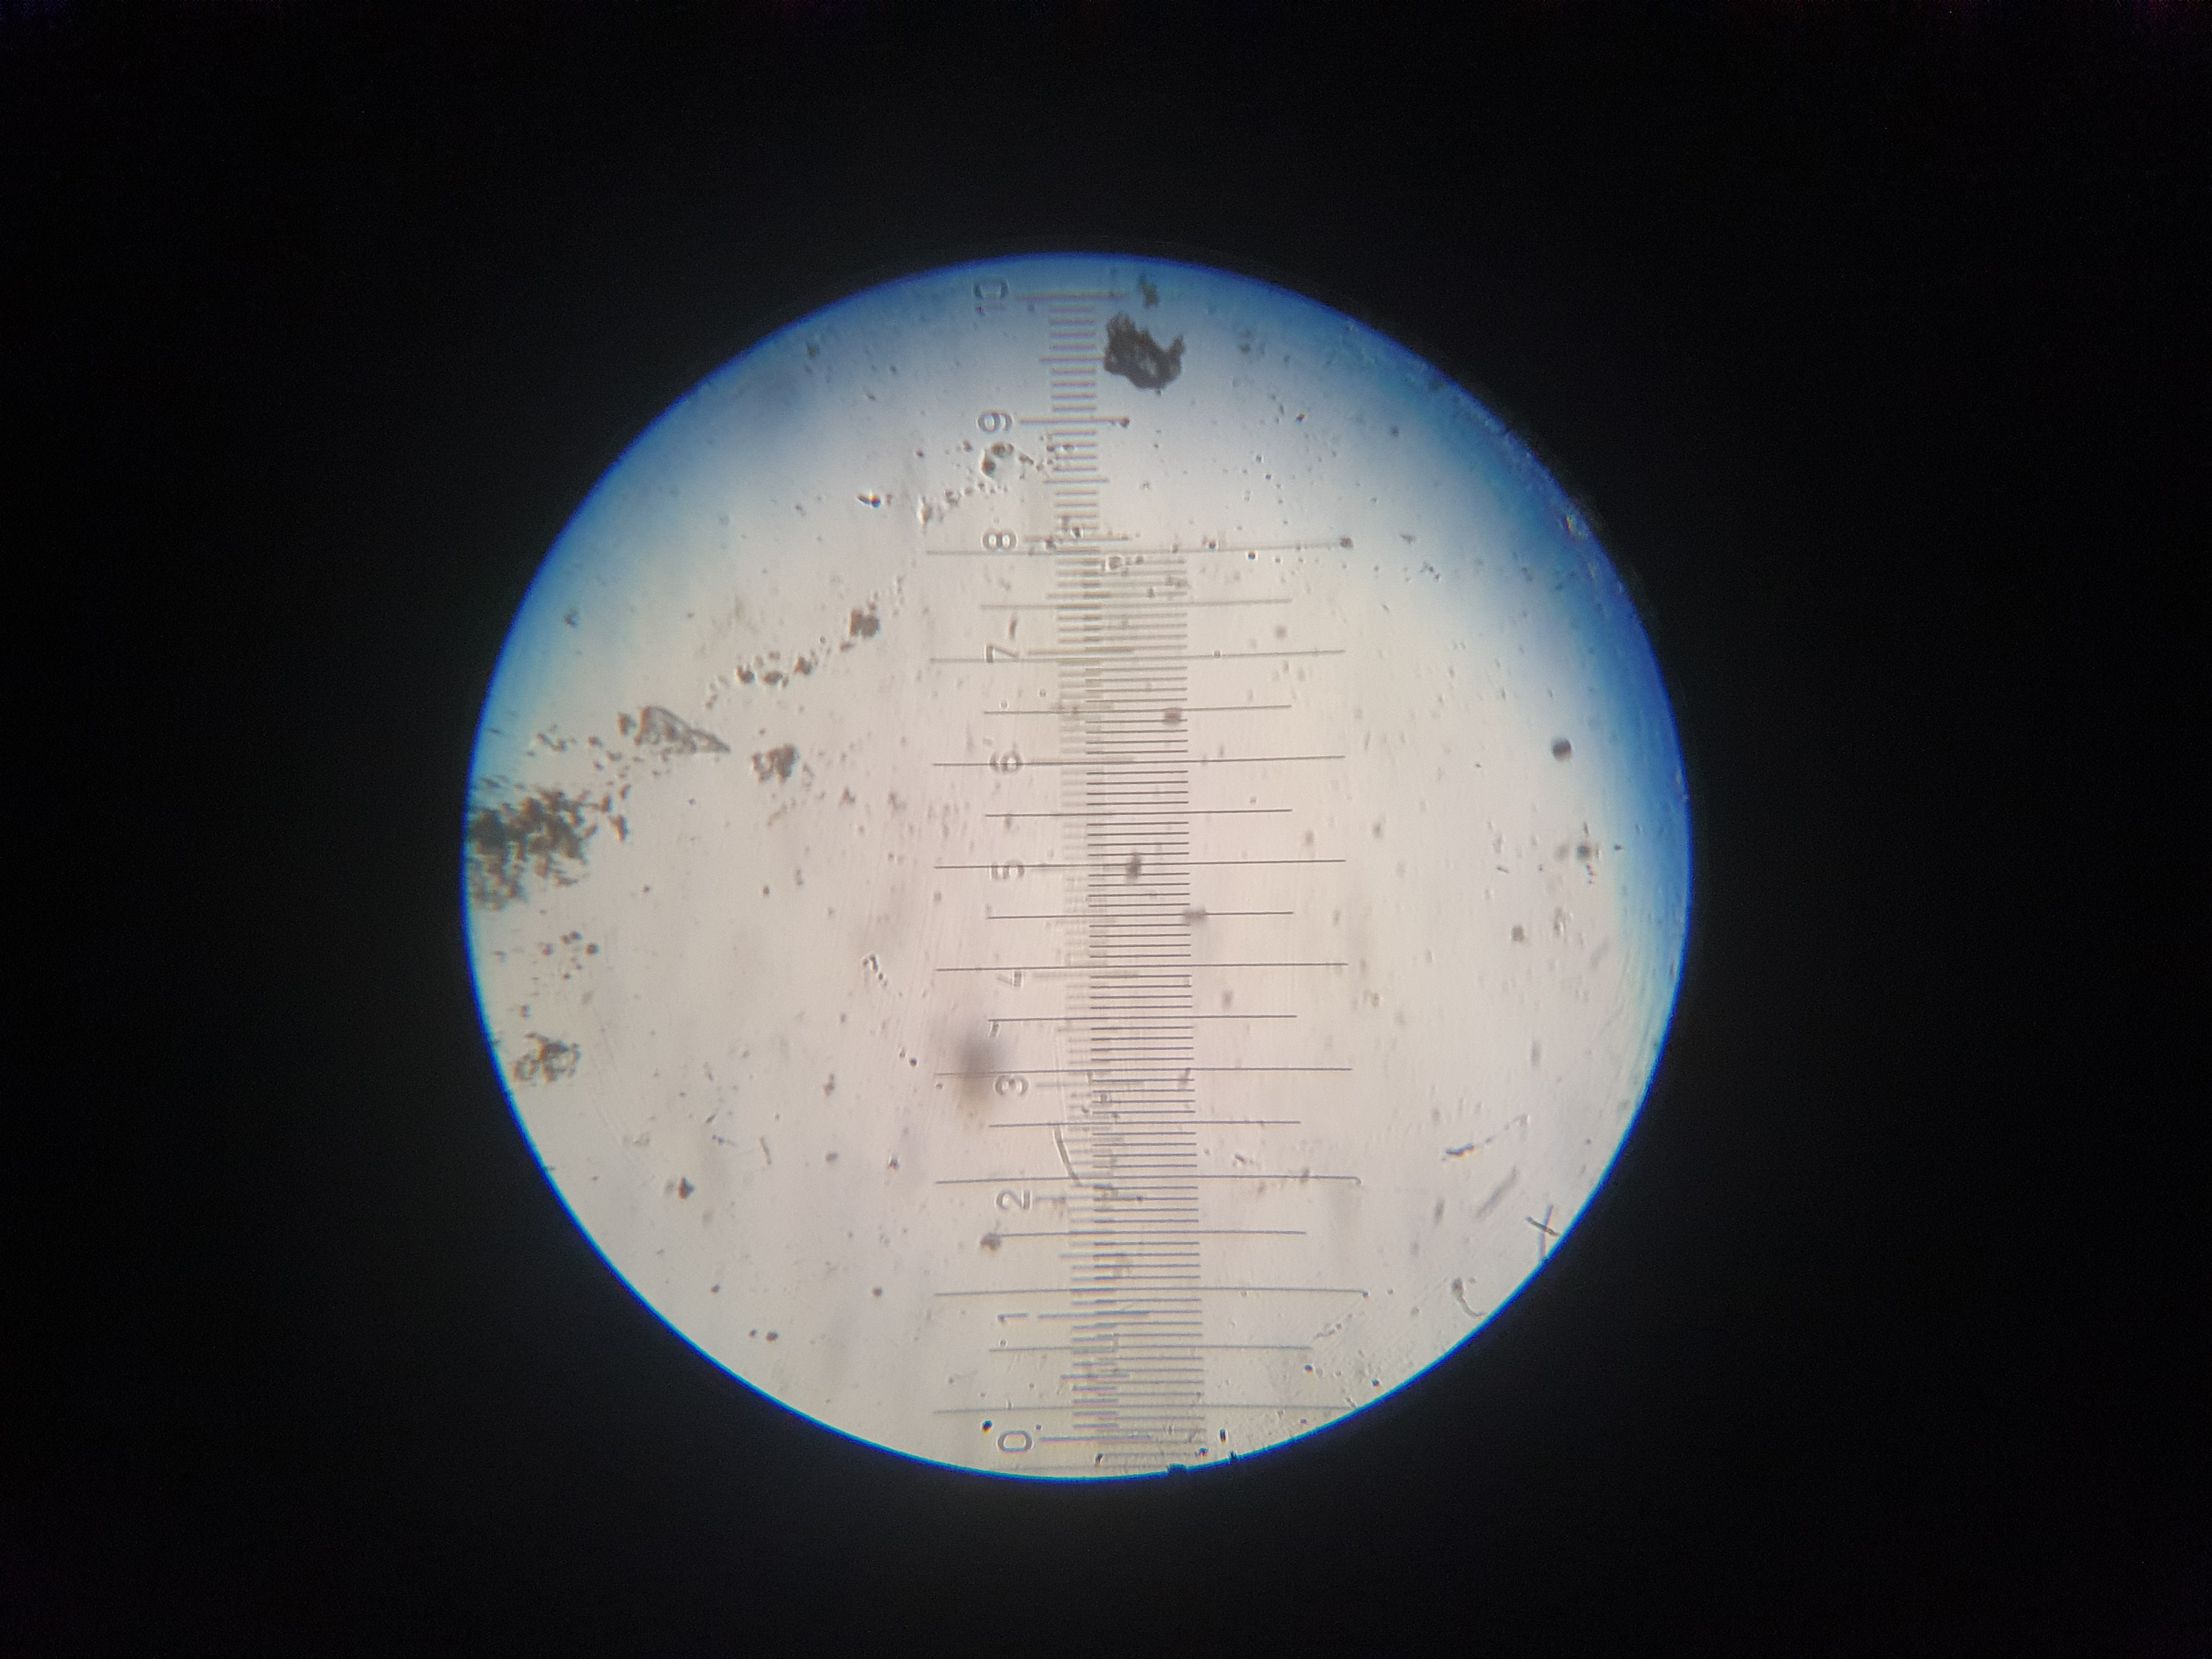
\includegraphics[width=0.5\linewidth, angle=0]{nudes/Aufsatz.jpg}
        \caption{Aufsatz mit halbdurchlässigem Spiegel}
        \label{fig:Aufsatz}
    \end{figure}        


\section{Geräteliste} %jo holt a listn ------------------------------

    \begin{table}[H]
        \centering
        \caption{Im Versuch verwendete Geräte und Utensilien.}
        \label{tab:geraete}
        \begin{tabular}{| l | l | l | l |}
            \hline
            Gerät & Gerätenummer  & Unsicherheit \\
            \hline
            Altes Mikroskop mit Vergleichsskala & {n.a} & {n.a} \\
            Neues Mikroskop mit Vergleichsskala & Zeiss Primostar 3 & {n.a} \\
            Aufsatz mit halbdurchlässigem Spiegel & {n.a} & {n.a} \\
            Objekt mit aufgedruckter Messskala & {n.a} & {n.a} \\
            Proben (Gitter, Haare - Melissa Eberhard) & {n.a} & {n.a} \\
            \hline
        \end{tabular}
    \end{table}


\section{Versuchsdurchführung \& Messergebnisse} %nachvollziehbar und klar dargestellt ------------------------------

Die Unsicherheiten der Werte der Messskalen wurden je mit $\pm$ 1 mm angenommen.

Der erste Teil des Versuches besteht aus der Bestimmung der Gesamt- und Objektivvergrößerung des alten Mikroskopes.
Hierfür wurde eine Probe mit einer kleinen (0.01 mm Schritte) Messskala unter das Mikroskop gelegt. 
Mit Hilfe des Aufsatzes kann nun die Skala unter dem Mikroskop mit der Skala hinter dem Mikroskop verglichen werden (Prinzip ersichtlich in Abbildung \ref{fig:Aufsatz}). \newline

\noindent
Legt man eine der beiden Skalen als Eins fest, so kann die andere Skala im Verhältnis dazu durch abzählen der kleinen Striche, welche in einen großen der anderen Skala passen, ermittelt werden.
Um Fehler, insbesondere Parallaxenfehler, zu minimieren, wurden jeweils drei verschiedene Messungen aus leicht geänderten Blickwinkeln notiert.
Durch adjustieren der Tubuslänge am Mikroskop können so verschiedene Vergößerungsdaten gesammelt werden, welche in folgenden Tabellen festgehalten wurden.

\begin{table}[H]
    \centering
    \caption{Messwerte Tubuslänge 20.1 cm}
    \label{tab:messwerteTB20}
    \begin{tabular}{| l | l | l |}
        \hline
        Nr.   & Vergleichsskala hinter Mikroskop [mm] $\pm$ 1  & Messkala am Objekt [mm] $\pm$ 1 \\
        \hline
        1 & 10 & 0.12 \\
        2 & 10 & 0.12 \\
        3 & 10 & 0.12 \\
        \hline
        Avg. & 10 & 0.12 \\
        \hline
    \end{tabular}
\end{table}

\begin{table}[H]
    \centering
    \caption{Messwerte Tubuslänge 19.1 cm}
    \label{tab:messwerteTB19}
    \begin{tabular}{| l | l | l |}
        \hline
        Nr.   & Vergleichsskala hinter Mikroskop [mm] $\pm$ 1 & Messkala am Objekt [mm] $\pm$ 1 \\
        \hline
        1 & 10 & 0.13 \\
        2 & 10 & 0.13 \\
        3 & 10 & 0.12 \\
        \hline
        Avg. & 10 & 0.127 \\
        \hline
    \end{tabular}
\end{table}

\begin{table}[H]
    \centering
    \caption{Messwerte Tubuslänge 17.1 cm}
    \label{tab:messwerteTB17}
    \begin{tabular}{| l | l | l |}
        \hline
        Nr.   & Vergleichsskala hinter Mikroskop [mm] $\pm$ 1 & Messkala am Objekt [mm] $\pm$ 1 \\
        \hline
        1 & 10 & 0.14 \\
        2 & 10 & 0.14 \\
        3 & 10 & 0.14 \\
        \hline
        Avg. & 10 & 0.14 \\
        \hline
    \end{tabular}
\end{table}

\begin{table}[H]
    \centering
    \caption{Messwerte Tubuslänge 16.1 cm}
    \label{tab:messwerteTB16}
    \begin{tabular}{| l | l | l |}
        \hline
        Nr.   & Vergleichsskala hinter Mikroskop [mm] $\pm$ 1 & Messkala am Objekt [mm] $\pm$ 1\\
        \hline
        1 & 10 & 0.16 \\
        2 & 10 & 0.15 \\
        3 & 10 & 0.15 \\
        \hline
        Avg. & 10 & 0.157 \\
        \hline
    \end{tabular}
\end{table}

\begin{table}[H]
    \centering
    \caption{Messwerte Tubuslänge 14.1 cm}
    \label{tab:messwerteTB14}
    \begin{tabular}{| l | l | l |}
        \hline
        Nr.   & Vergleichsskala hinter Mikroskop [mm] $\pm$ 1 & Messkala am Objekt [mm] $\pm$ 1 \\
        \hline
        1 & 10 & 0.17 \\
        2 & 10 & 0.17 \\
        3 & 10 & 0.17 \\
        \hline
        Avg. & 10 & 0.17 \\
        \hline
    \end{tabular}
\end{table}

\noindent
Zur Bestimmung der Okularvergrößerung wurden diese Messvorgänge wiederholt, jedoch kam jetzt ein Okular mit 10-facher Vergrößerung zum Einsatz. 
Außerdem enthält dieses Okular eine eigene Messskala, welche mit der Skala am Objekt verglichen wurde.
Die Messwerte wurden wiederum in Tabellen gesammelt.

\begin{table}[H]
    \centering
    \caption{Messwerte Tubuslänge 20.1 cm}
    \label{tab:10XmesswerteTB20}
    \begin{tabular}{| l | l | l |}
        \hline
        Nr.   & Vergleichsskala im Okular [mm] $\pm$ 1 & Messkala am Objekt [mm] $\pm$ 1 \\
        \hline
        1 & 0.1 & 9 \\
        2 & 0.1 & 9 \\
        3 & 0.1 & 9 \\
        \hline
        Avg. & 0.1 & 9 \\
        \hline
    \end{tabular}
\end{table}

\begin{table}[H]
    \centering
    \caption{Messwerte Tubuslänge 19.1 cm}
    \label{tab:10XmesswerteTB19}
    \begin{tabular}{| l | l | l |}
        \hline
        Nr.   & Vergleichsskala im Okular [mm] $\pm$ 1 & Messkala am Objekt [mm] $\pm$ 1 \\
        \hline
        1 & 0.1 & 10 \\
        2 & 0.1 & 10 \\
        3 & 0.1 & 11 \\
        \hline
        Avg. & 0.1 & 10.3 \\
        \hline
    \end{tabular}
\end{table}

\begin{table}[H]
    \centering
    \caption{Messwerte Tubuslänge 17.1 cm}
    \label{tab:10XmesswerteTB17}
    \begin{tabular}{| l | l | l |}
        \hline
        Nr.   & Vergleichsskala im Okular [mm] $\pm$ 1 & Messkala am Objekt [mm] $\pm$ 1 \\
        \hline
        1 & 0.1 & 9 \\
        2 & 0.1 & 9 \\
        3 & 0.1 & 8 \\
        \hline
        Avg. & 0.1 & 8.7 \\
        \hline
    \end{tabular}
\end{table}

\begin{table}[H]
    \centering
    \caption{Messwerte Tubuslänge 16.1 cm}
    \label{tab:10XmesswerteTB16}
    \begin{tabular}{| l | l | l |}
        \hline
        Nr.   & Vergleichsskala im Okular [mm] $\pm$ 1 & Messkala am Objekt [mm] $\pm$ 1 \\
        \hline
        1 & 0.1 & 8 \\
        2 & 0.1 & 8 \\
        3 & 0.1 & 8 \\
        \hline
        Avg. & 0.1 & 8 \\
        \hline
    \end{tabular}
\end{table}

\begin{table}[H]
    \centering
    \caption{Messwerte Tubuslänge 14.1 cm}
    \label{tab:10XmesswerteTB14}
    \begin{tabular}{| l | l | l |}
        \hline
        Nr.   & Vergleichsskala im Okular [mm] $\pm$ 1 & Messkala am Objekt [mm] $\pm$ 1 \\
        \hline
        1 & 0.1 & 8 \\
        2 & 0.1 & 7 \\
        3 & 0.1 & 7 \\
        \hline
        Avg. & 0.1 & 7.7 \\
        \hline
    \end{tabular}
\end{table}

\noindent
Um die Gesamtvergrößerung des neuen Mikroskopes zu bestimmen wurde mit der gleichen Herangehensweiße gearbeitet, jedoch sind hier die Objektivvergrößerungswerte auf den jeweiligen Objektiven ersichtlich und somit bekannt. 

\begin{table}[H]
    \centering
    \caption{Messwerte 4x Objektivvergrößerung}
    \label{tab:messwerteNM4x}
    \begin{tabular}{| l | l | l |}
        \hline
        Nr.   & Vergleichsskala ober Mikroskop [mm] $\pm$ 1 & Messkala am Objekt [mm] $\pm$ 1 \\
        \hline
        1 & 10 & 0.24 \\
        2 & 10 & 0.24 \\
        3 & 10 & 0.25 \\
        \hline
        Avg. & 1 & 0.247 \\
        \hline
    \end{tabular}
\end{table}

\begin{table}[H]
    \centering
    \caption{Messwerte 10x Objektivvergrößerung}
    \label{tab:messwerteNM10x}
    \begin{tabular}{| l | l | l |}
        \hline
        Nr.   & Vergleichsskala ober Mikroskop [mm] $\pm$ 1 & Messkala am Objekt [mm] $\pm$ 1 \\
        \hline
        1 & 10 & 0.090 \\
        2 & 10 & 0.091 \\
        3 & 10 & 0.090 \\
        \hline
        Avg. & 1 & 0.091 \\
        \hline
    \end{tabular}
\end{table}

\begin{table}[H]
    \centering
    \caption{Messwerte 40x Objektivvergrößerung}
    \label{tab:messwerteNM40x}
    \begin{tabular}{| l | l | l |}
        \hline
        Nr.   & Vergleichsskala ober Mikroskop [mm] $\pm$ 1 & Messkala am Objekt [mm] $\pm$ 1 \\
        \hline
        1 & 10 & 0.0250 \\
        2 & 10 & 0.0240 \\
        3 & 10 & 0.0240 \\
        \hline
        Avg. & 1 & 0.0247 \\
        \hline
    \end{tabular}
\end{table}

\noindent
Weiters wurden am Ende der Durchführung Bilder von verschiedenen Proben mittels Computersoftware  aufgenommen, welche in der Auswertung noch gezeigt und beschrieben werden.


\section{Auswertung und Unsicherheitsanalyse} %Nicht nur zahlen angeben ------------------------------

In der Auswertung werden zur erhöhten Genauigkeit durchgehend ungerundete Werte bis zu den Endergebnissen verwendet und nur zur Darstellung gerundet. \\
Zur Berechnung der Unsicherheiten wird, wenn nicht anders angegeben, die Größtunsicherheitsmethode verwendet.

\subsection{Objektivvergrößerung altes Mikroskop und Diagramm}
Zur Bestimmung der Objektivvergrößerung des alten Mikroskopes wurden die Durchschnittswerte aus den Tabellen \ref{tab:messwerteTB20}-\ref{tab:messwerteTB14} verwendet.
Durch einsetzen dieser in Formel \ref{eq:VergrößerungAM} bzw. Formel \ref{eq:Unsicherheit_VergrößerungAM} für die Unsicherheiten ergeben sich folgende Werte für die Vergrößerung:

\begin{table}[H]
    \centering
    \caption{Gesamtvergrößerungen der jeweiligen Tubuslängen}
    \label{tab:Gesamtvergrößerung}
    \begin{tabular}{| l | l | l |}
        \hline
        Nr.   & Tubuslänge [cm]  & Vergrößerung [] \\
        \hline
        1 & 20.1 & 83.40 $\pm$ 627.90 \\
        2 & 19.1 & 78.80 $\pm$ 686.60 \\
        3 & 17.1 & 71.50 $\pm$ 503.10 \\
        4 & 16.1 & 63.70 $\pm$ 399.40 \\
        5 & 14.1 & 58.92 $\pm$ 380.14 \\
        \hline
    \end{tabular}
\end{table}

\noindent
Durch das grafische Darstellen dieser Werte in einem Diagramm und einer Ausgleichsgerade in qti-Plot lässt sich folgender Plot erkennen.

\begin{figure}[H]
    \centering
    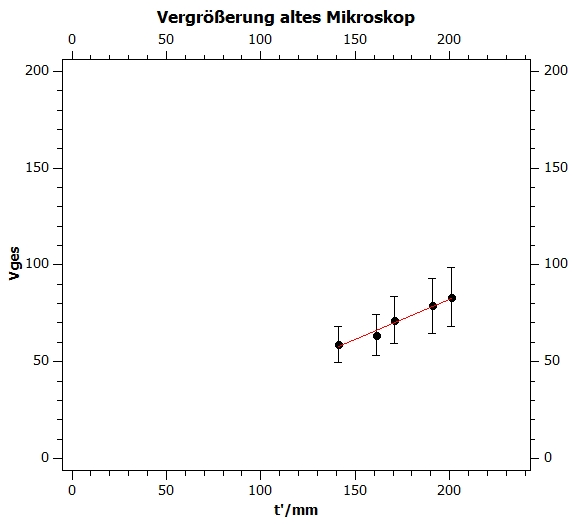
\includegraphics[width=0.6\linewidth, angle=0]{nudes/VergrößerungAltesMik.jpg}
    \caption{Vergrößerung in Abhängigkeit der Tubuslänge in qti-Plot}
    \label{fig:VergrößerungDiagramm}
\end{figure}

\noindent
Für die Ausgleichsgerade ergibt sich folgende Funktion $V(t') = 4.22*t' - 1.69$. Setzt man die Funktion gleich null, so erhält man durch umformen den Wert für x = 0.4. \newline

\noindent 
Zur Bestimmung der Objektivvergrößerung wurde dann ein anderes Okular verwendet, welche eine bekannte Vergrößerung von 10 $\pm$ 0 besitzt. 
Mit den Gesamtvergrößerungen, welche mittels Formel \ref{eq:VergrößerungAM10x} bzw. \ref{eq:Unsicherheit_VergrößerungAM10x} und den Daten aus den Tabellen \ref{tab:10XmesswerteTB20}-\ref{tab:10XmesswerteTB14} berechnet wurden, konnten mit Hilfe von Formel \ref*{eq:Gesamtvergrößerung} bzw. \ref{eq:Unsicherheit_Gesamtvergrößerung} die Objektivvergrößerungen der jeweiligen Tubuslängen ermittelt werden.

\begin{table}[H]
    \centering
    \caption{Berechnete Objektivvergrößerungen der jeweiligen Tubuslängen}
    \label{tab:Objektivvergrößerungen}
    \begin{tabular}{| l | l | l | l |}
        \hline
        Nr.   & Tubuslänge [cm]  & Gesamtvergrößerung [] & Objektivvergrößerung [] \\
        \hline
        1 & 20.1 & 90 $\pm$ 890 & 9.0 $\pm$ 89 \\
        2 & 19.1 & 103 $\pm$ 1020 & 10.3 $\pm$ 102 \\
        3 & 17.1 & 87 $\pm$ 860 & 8.7 $\pm$ 86 \\
        4 & 16.1 & 80 $\pm$ 790 & 8.0 $\pm$ 79 \\
        5 & 14.1 & 77 $\pm$ 760 & 7.7 $\pm$ 76 \\
        \hline
    \end{tabular}
\end{table}


\subsection{Okularvergrößerung}

Mit Hilfe von Formel \ref{eq:Gesamtvergrößerung} bzw. \ref{eq:Unsicherheit_Gesamtvergrößerung} lässt sich außerdem die Okularvergrößerung des verwendeten Okulars bei den Werten von Tabelle \ref{tab:messwerteTB20}-\ref{tab:messwerteTB14} ermitteln.

\begin{table}[H]
    \centering
    \caption{Berechnete Okularvergrößerung der jeweiligen Tubuslängen}
    \label{tab:Okularvergrößerungen}
    \begin{tabular}{| l | l | l | l | l |}
        \hline
        Nr.   & Tubuslänge [cm]  & Gesamtvergrößerung [] & Objektivvergrößerung [] & Okularvergrößerung [] \\
        \hline
        1 & 20.1 & 83.40 $\pm$ 627.90 & 9.0 $\pm$ 89 & 9.3 $\pm$ 636.7 \\
        2 & 19.1 & 78.80 $\pm$ 686.60 & 10.3 $\pm$ 102 & 7.7 $\pm$ 519.9 \\
        3 & 17.1 & 71.50 $\pm$ 503.10 & 8.7 $\pm$ 86 & 8.22 $\pm$ 485.14 \\
        4 & 16.1 & 63.70 $\pm$ 399.40 & 8.0 $\pm$ 79 & 8.0 $\pm$ 407.4 \\
        5 & 14.1 & 58.90 $\pm$ 380.14 & 7.7 $\pm$ 76 & 7.7 $\pm$ 387.6 \\
        \hline
    \end{tabular}
\end{table}

\subsection{Objektivbrennweite}

Die Objektivbrennweiten ergeben sich mit Formel \ref{eq:Objektivbrennweite} bzw. \ref{eq:Unsicherheit_Objektivbrennweite} und den Werten für die Objektivvergrößerungen aus Tabelle \ref{tab:Objektivvergrößerungen}.

\begin{table}[H]
    \centering
    \caption{Berechnete Objektivvergrößerungen der jeweiligen Tubuslängen}
    \label{tab:Objektivbrennweiten}
    \begin{tabular}{| l | l | l | l |}
        \hline
        Nr.   & Tubuslänge [cm]  & Objektivvergrößerung [] & Objektivbrennweite [mm] \\
        \hline
        1 & 20.1 & 9.0 $\pm$ 89 & 22.4 $\pm$ 220.9 \\
        2 & 19.1 & 10.3 $\pm$ 102 & 18.6 $\pm$ 183.7 \\
        3 & 17.1 & 8.7 $\pm$ 86 & 19.7 $\pm$ 194.3 \\
        4 & 16.1 & 8.0 $\pm$ 79 & 20.2 $\pm$ 198.8 \\
        5 & 14.1 & 7.7 $\pm$ 76 & 18.4 $\pm$ 180.8 \\
        \hline
    \end{tabular}
\end{table}

\subsection{Gesamtvergrößerung neues Mikroskop}

Für die Gesamtvergrößerungen des neuen Mikroskopes der einzelnen Objektivvergrößerungen wird wiederum die Formel \ref{eq:Gesamtvergrößerung} verwendet.
Gemeinsam mit den Durchschnittswerten der Gesamtvergrößerung aus Tabellen \ref{tab:messwerteNM4x}-\ref{tab:messwerteNM40x} kann mittels Formel \ref{eq:VergrößerungNM} bzw. \ref{eq:Unsicherheit_VergrößerungNM} auf die Gesamtvergrößerung geschlossen werden.

\begin{table}[H]
    \centering
    \caption{Berechnete Objektivvergrößerungen der jeweiligen Tubuslängen}
    \label{tab:GesamtvergrößerungNM}
    \begin{tabular}{| l | l | l | l |}
        \hline
        Nr.   & Objektivvergrößerung [] & Gesamtvergrößerung berechnet [] & Gesamtvergrößerung gerundet [] \\
        \hline
        1 & 4 & 40.5 $\pm$ 159.9 & 40 \\
        2 & 10 & 109.9 $\pm$ 1196.6 & 100 \\
        3 & 40 & 404.9 $\pm$ 16350 & 400 \\
        \hline
    \end{tabular}
\end{table}



\subsection{Vergleich Mikroskope alt/neu}

Vergleicht man die beiden Mikroskope miteinander, so sollte einem jedem sofort ins Auge fallen, dass das ältere Mikroskop ihrem modernerem Gegenstück optisch, als auch praktisch etwas hinterherhinkt.
Zum einen gibt es natürlich den großen Unterschied, dass man beim alten Mirkoskop die Tubuslänge manuell einstellen kann. Dafür gibt es beim neuen Mikroskop die Möglichkeit, die Objektive zu wechseln. \newline

\noindent
Das neue Mikroskop weißt außerdem ein kompakteres und einfacheres Design auf, was sich vor allem beim Bestimmen der Vergrößerungen als vorteilhafter herausgestellt hat. \newline

\noindent
Mit Hilfe der folgenden Tabelle lassen sich nun die Vergrößerungsleistungen der beiden Mikroskope vergleichen.

\begin{table}[H]
    \centering
    \caption{Berechnete Objektivvergrößerungen der jeweiligen Tubuslängen}
    \label{tab:Okularvergrößerungen}
    \begin{tabular}{| l | l | l |}
        \hline
           & Mikroskop neu & Mikroskop alt \\
        \hline
        max. gemessene Gesamtvergrößerung & 400 & 103 \\
        min. gemessene Gesamtvergrößerung & 40 & 77 \\
        \hline
    \end{tabular}
\end{table}

\noindent
Mit dem neuen Mikroskop lässt sich ein wesentlich größerer Vergrößerungsbereich erzielen. 
Beim modernen Forschen sollte das neue Mikroskop mit Sicherheit für die meisten Untersuchungsaufgaben das bessere und handlichere Hilfsmittel darstellen.
Es schadet jedoch sicherlich nicht, sich auch mit dem älterem Mikroskop auseinanderzusetzen, da auf digitale Technologie nicht immer Verlass ist, vor allem wenn der Strom fehlt.


\subsection{Untersuchung von Proben (digital)}

Im letzten Punkt der Aufgabenstellung sollten Proben mit dem neuen Mikroskop untersucht und vermessen werden. \newline

\noindent
Hierfür wurden ein altes Transmissionsgitter und eine Graphenprobe im wahrsten Sinne des Wortes unter die Lupe bzw. unter das Mikroskop genommen.
Die Resultate wurden digital am Computerbildschirm dargestellt und zur weiteren Untersuchung auf

\begin{itemize}
    \item Transmissionsgitter: Liniendichte
    \item Graphenprobe: Graphenbedeckung der Oberfläche
    \item Haarprobe 
\end{itemize}

\noindent
abfotografiert. Die Ergebnisse sind in den folgenden Abbildungen zu sehen:

\begin{figure}[H]
    \centering
    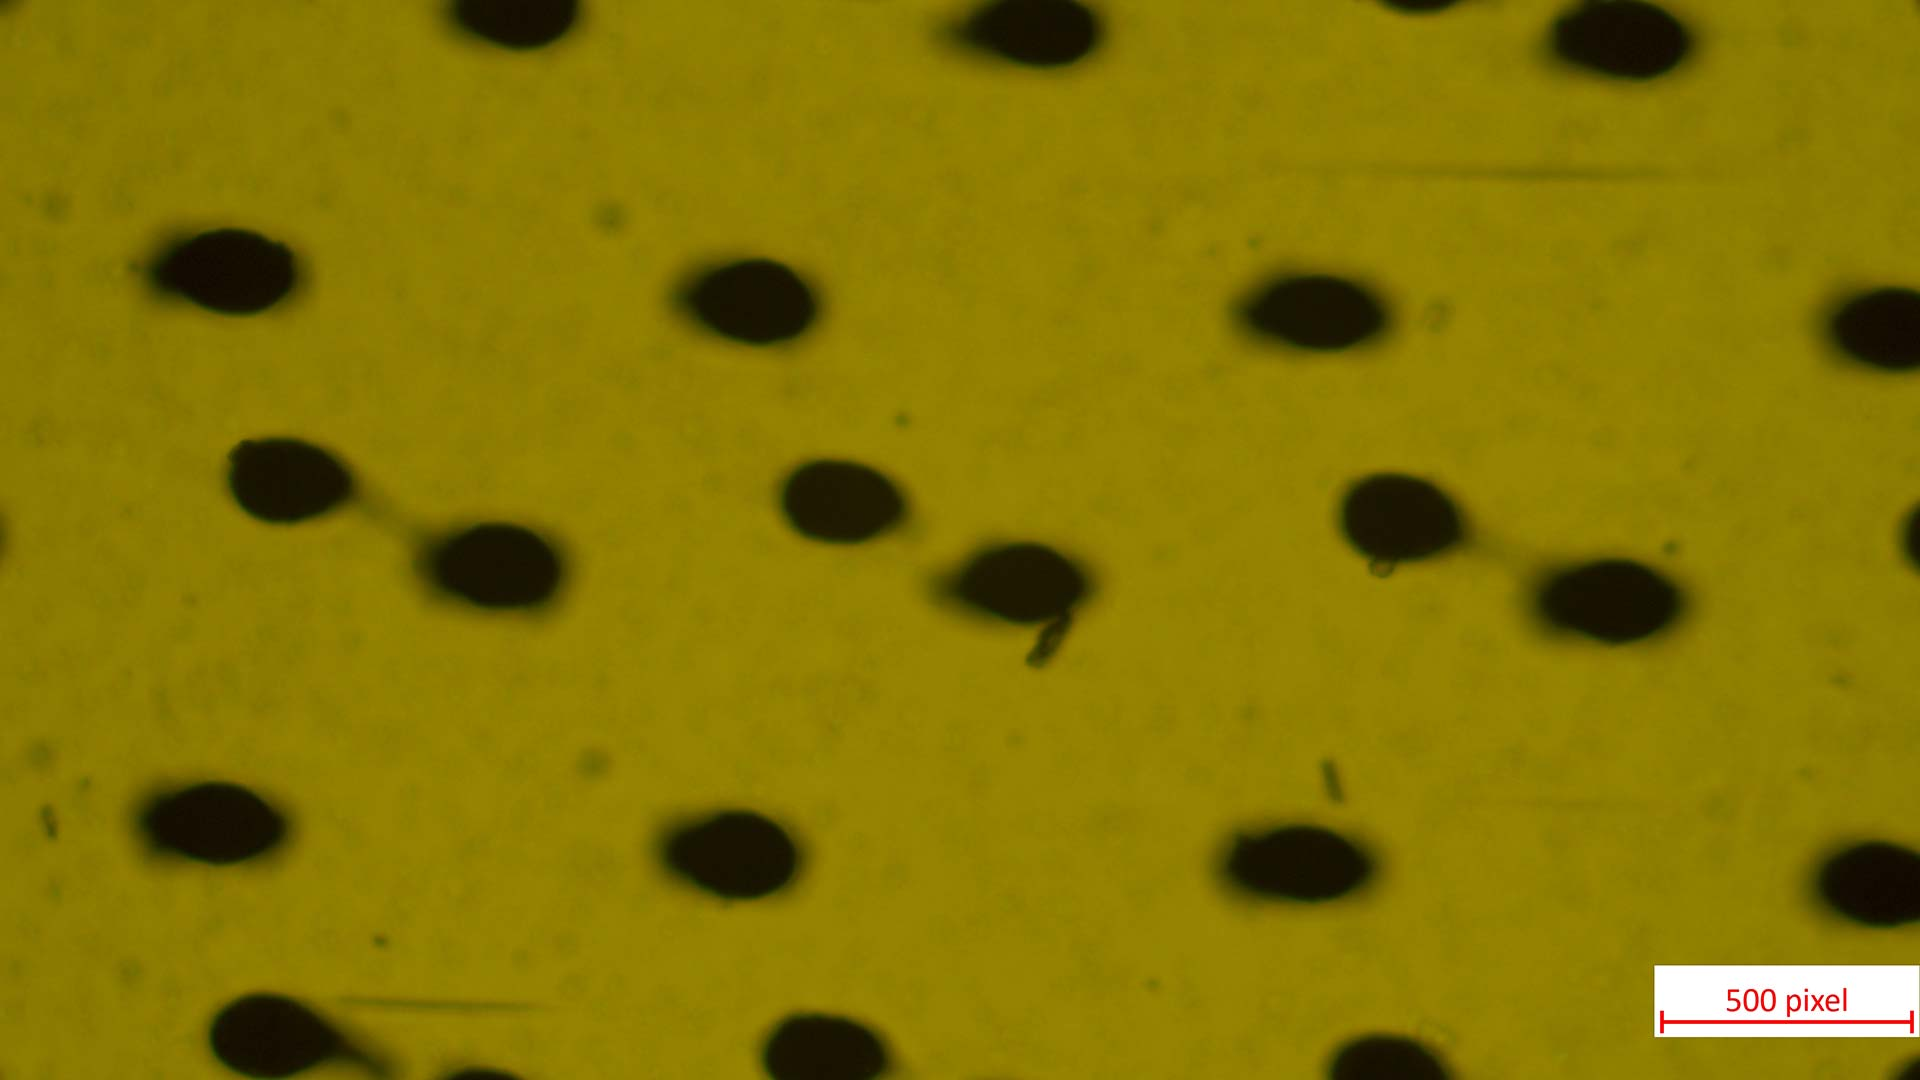
\includegraphics[width=0.5\linewidth, angle=0]{nudes/mikro/Snap_001.jpg}
    \caption{Transmissionsgitter 15$\%$}
    \label{fig:Transmissionsgitter15}
\end{figure}

\begin{figure}[H]
    \centering
    \includegraphics[width=0.5\linewidth, angle=0]{nudes/mikro/Snap_004.jpg}
    \caption{Transmissionsgitter 50$\%$}
    \label{fig:Transmissionsgitter50}
\end{figure}

\begin{figure}[H]
    \centering
    \includegraphics[width=0.5\linewidth, angle=0]{nudes/mikro/Snap_002.jpg}
    \caption{Transmissionsgitter 100$\%$}
    \label{fig:Transmissionsgitter100}
\end{figure}

\begin{figure}[H]
    \centering
    \includegraphics[width=0.5\linewidth, angle=0]{nudes/mikro/Snap_003.jpg}
    \caption{Graphenprobe}
    \label{fig:graphenprobe}
\end{figure}

\begin{figure}[H]
    \centering
    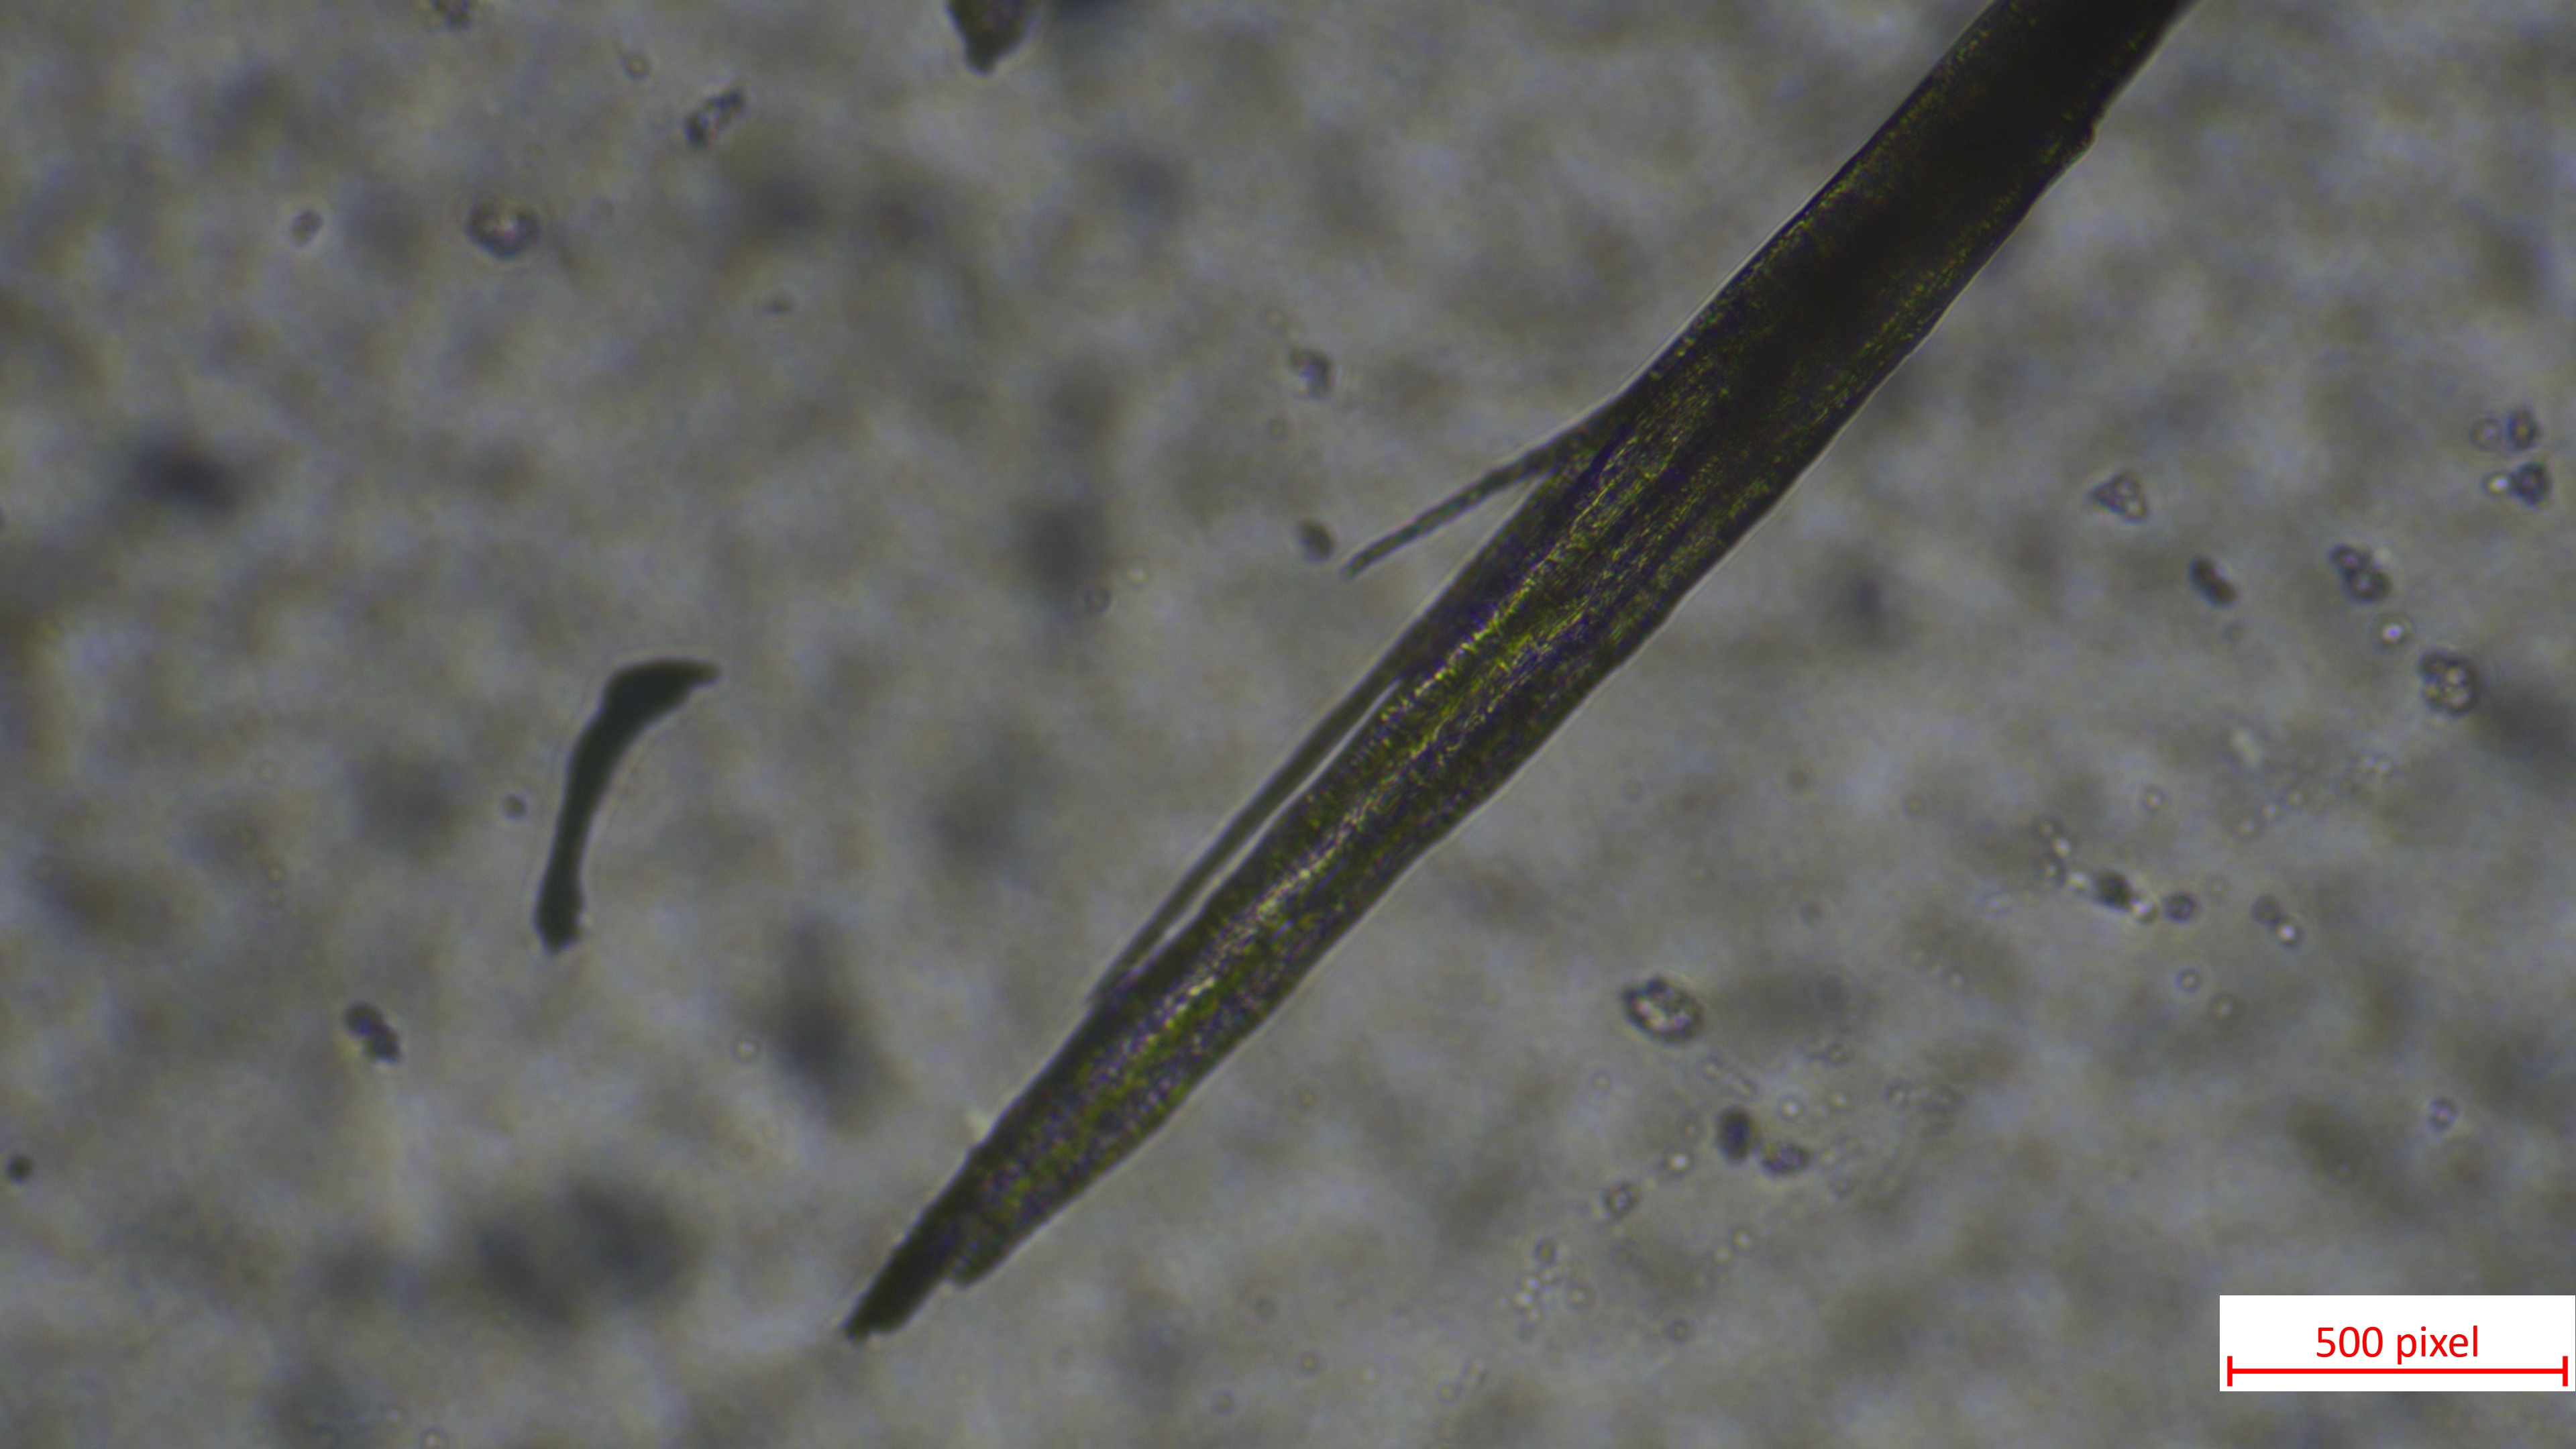
\includegraphics[width=0.5\linewidth, angle=0]{nudes/mikro/Snap_005.jpg}
    \caption{Haarprobe}
    \label{fig:haarprobe}
\end{figure}

\begin{table}[H]
    \centering
    \caption{Probenaufgaben}
    \label{tab:Probenaufgabe}
    \begin{tabular}{| l | l | l |}
        \hline
        Objekt & Aufgabe & Ergebnis \\
        \hline
        Transmissionsgitter 15$\%$ & Liniendichte &  \\
        Transmissionsgitter 50$\%$ & Liniendichte &  \\
        Transmissionsgitter 100$\%$ & Liniendichte &  \\
        Graphenprobe & Graphenbedeckung &  \\
        Haarprobe & & \\
        \hline
    \end{tabular}
\end{table}


\section{Diskussion} %diskussion der Unsicherheiten und Ergebnisse und evtl. verlgeich mit Literatur ------------------------------

Ein Luftthermometer ist ein unabdingbares Hilfsmittel in der Forschung. 

\subsection{Objektivvergrößerung altes Mikroskop}

Die Gesamtvergrößerungen von Mikroskopen hängt von der Zusammensetzung aus Okular- und Objektivvergrößerung ab.
Da die Vergrößerung des eingebauten Objektives nicht bekannt ist, lässt sich auch kein literarischer Wert für die Gesamtvergrößerung anführen. \newline

\noindent
Eine Verlängerung der Tubuslänge führt jedooch meist zu einer Vergrößerung, was sich auch bei den genannten Messergebnissen bemerkbar macht. 
Dies ist möglicherweiße ein Indiz für eine richtige Durchführung des Experimentes. 

\subsection{Okularvergrößerung}

Selbiges Problem wie bei der Objektivvergrößerung lässt sich auch bei der Okularvergrößerung finden, jedoch sinkt auch hier die Vergrößerung mit der Tubuslänge. 


\subsection{Objektivbrennweite}

In der Mikroskopie liegen die Objektivbrennweiten meist zwischen 2mm und 20mm oder mehr. Diese Werte decken sich ebenfalls mit den berechneten Brennweiten aus Tabelle \ref{tab:Objektivbrennweiten}.


\subsection{Gesamtvergrößerung neues Mikroskop}

Die berechneten Werte der Gesamtvergrößerung aus Tabelle \ref{tab:GesamtvergrößerungNM} legen ein verwendetes Okular mit einer Vergrößerung von 10 nahe, was ebenfalls auf die korrekte Versuchsdurchführung hinweist.


\section{Zusammenfassung} %klare, übersichtliche vollständige beantwortung der Aufgabenstellung ------------------------------

Hier nocheinmal die Ergebnisse zusammengefasst.

\begin{table}[H]
    \centering
    \caption{Ergebnisse altes Mikroskop}
    \label{tab:ErgebnisseAM}
    \begin{tabular}{| l | l | l | l | l | l |}
        \hline
         & TL 21.1 & TL 19.1 & TL 17.1 & TL 16.1 & TL 14.1 \\
        \hline
        Gesamtvergrößerung & 83.4 & 78.8 & 71.5 & 63.7 & 58.9 \\
        Objektivvergrößerung & 9.0 & 10.3 & 8.7 & 8.0 & 7.7 \\
        Okularvergrößerung & 9.27 & 7.65 & 8.22 & 7.97 & 7.65 \\
        Objektivbrennweite & 22.3 & 18.6 & 19.7 & 20.2 & 18.4 \\
        \hline
    \end{tabular}
\end{table}

\begin{table}[H]
    \centering
    \caption{Ergebnisse neues Mikroskop}
    \label{tab:ErgebnisseNM}
    \begin{tabular}{| l | l | l | l |}
        \hline
         & Obj 4x & Obj 10x & Obj. 40x \\
        \hline
        Gesamtvergrößerung & 40 & 100 & 400 \\
        \hline
    \end{tabular}
\end{table}

\begin{figure}[H]
    \centering
    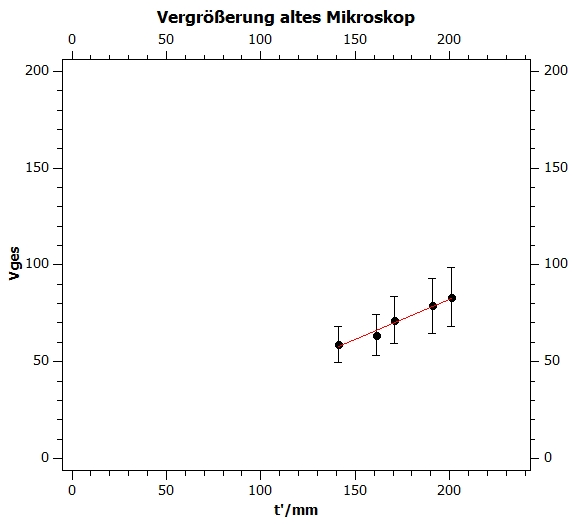
\includegraphics[width=0.6\linewidth, angle=0]{nudes/VergrößerungAltesMik.jpg}
    \caption{Vergrößerung in Abhängigkeit der Tubuslänge in qti-Plot}
    \label{fig:VergrößerungDiagramm}
\end{figure}



\printbibliography[heading=bibintoc]
\end{document}
